In this Section, we evaluate our system through a series of experiments on simple queries. We focus on just simple ones to emphasize the benefits of caching as a function of the particular operators involved in each query. For simplicity, we consider workloads composed by two queries only, and compute the running time of the Spark jobs associated to each query, with and without our cache-based multi-query optimization mechanism. Overall, our results indicate:

\begin{itemize}
	\item Roughly 50\% and 30\% improvement in aggregate query latencies for CSV and Parquet files respectively.
	\item Memory utilization is always better or equal than the naive approach.
\end{itemize}

In our graphs, we use the following notation:
\begin{itemize}
	\item R\_Job1, R\_Job2: job execution times, with no caching
	\item R\_Job1*, R\_Job2*: job execution times, with caching
	\item M\_R: Total memory utilization, in Bytes
	\item M\_D: Total disk utilization, in Bytes. This metric accounts for data that does not fit in RAM, and is spilled to disk by the Spark caching mechanism.
	\item M: total storage utilization, by the caching plan
	\item I: input size of the dataset, in terms of records.
\end{itemize}

Next, we first examine Filter and Project operations because they appear very frequently in data analysis, and are usually pushed as close as possible to the input by traditional query optimization techniques. Then, we consider the top-K problem and finally move to Filter and Project operations over very large amount of data.

\subsection{Filter-based queries}
The two queries are described by the logical plans depicted in Figure \ref{fig:query1_plans}. The top left and top right logical plans indicate that the two queries we consider read data from the same input relation, then apply a filter operation with two different predicates. The logical plan displayed at the bottom of the Figure is the result output by our multi-query optimizer: Job1* first reads the data from the input relation, then applies a Filter operator, with a combined predicate. Next, Job1* caches the filtered data and finally applies its own filter predicate to produce the output. The second job Job2*, reads directly its input data from the cache.

\begin{figure}[htbp]
   \centering
   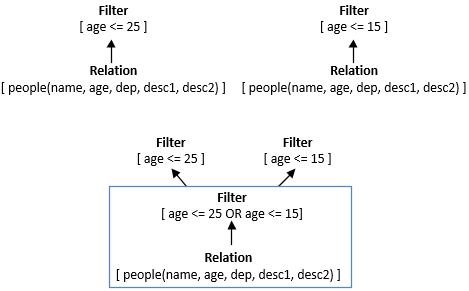
\includegraphics[scale=0.5]{figures/query1_cacheplan}
   \caption{Query and Cache plan for Filter-based queries.} 
   \label{fig:query1_plans}
\end{figure}

Next, in Figure \ref{fig:query1}, we show the individual and aggregate query latencies, with and without our optimization. We also show the impact of the input data format, considering both Parquet and CSV input files.

\begin{figure}[htbp]
	\centering
	\subfigure[Parquet]{
   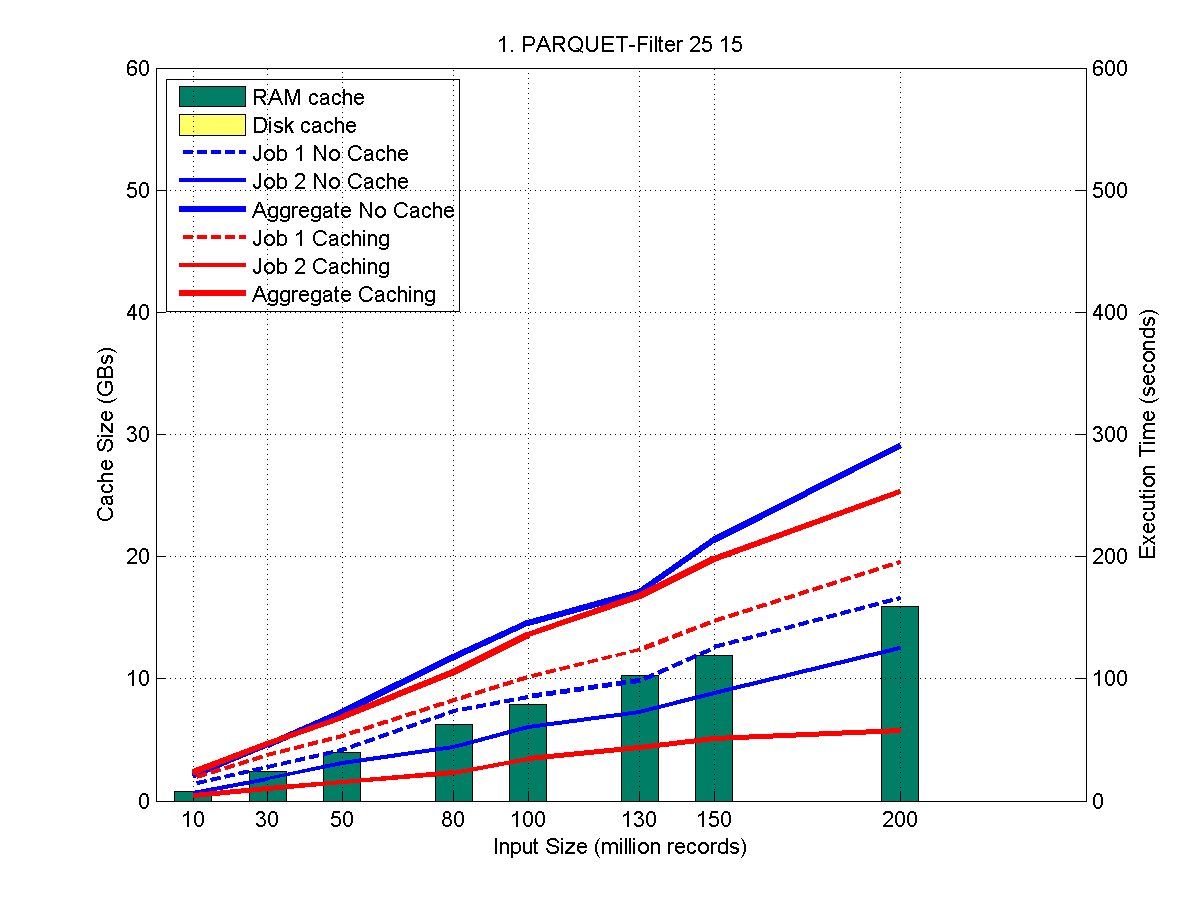
\includegraphics[scale=0.4]{figures/query1_parquet}
   \label{fig:query1_parquet}}

  	\subfigure[CSV]{
   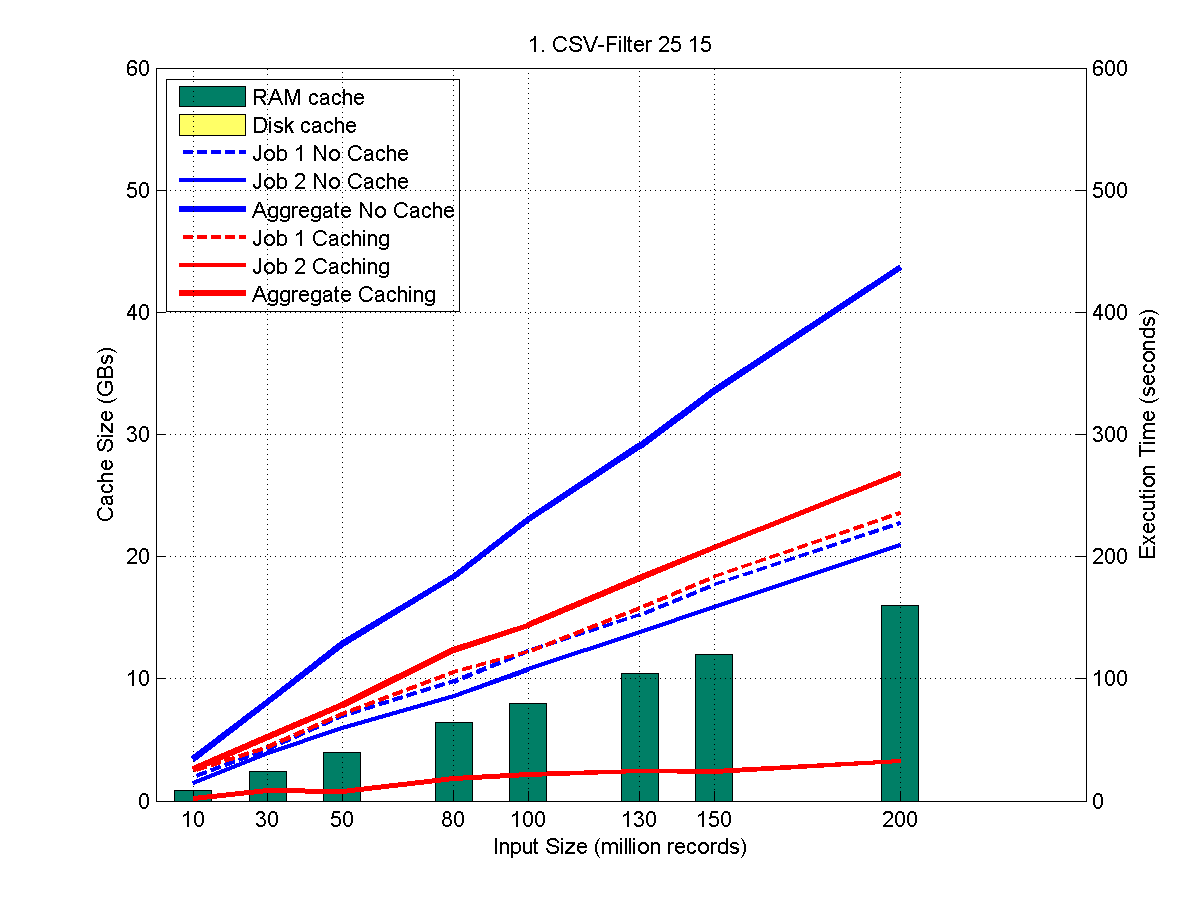
\includegraphics[scale=0.4]{figures/query1_csv}
   \label{fig:query1_csv}}

   \caption{Filter-based queries, query latencies and memory utilization.}
   \label{fig:query1}
\end{figure}

The first set of results indicate the multi-query optimizer works as expected: for both Parquet and CSV input format, the aggregate query latency for the two jobs is shorter with caching optimization. In details, we notice that Job1* runs slower than Job1: this is attributed to the cost of the caching operation. However, the difference in runtime between Job1* and Job1 is not the same for the case Parquet (noticeable different) and CSV (somehow equals). Additionally, the execution time of Job2* (which involves reading data from cache then writing data to disk) for both formats shows different pattern: when data is in Parquet format, Job2* benefits less from caching.

The cache size is roughly 25\% of the size of input data, for both the Parquet and CSV case. Our multi-query optimizer uses only 1/3 of the caching capacity (25\% of 200M records costs 16GB of cache size, which totals 45GB in our system).

Next, we consider a different set of filtering conditions, which are more stressful with respect to memory utilization. The queries we consider are less selective than the ones presented above, with filtering predicates as follows: \texttt{age <= 50} and \texttt{age <= 25}. Figure \ref{fig:query1_50} shows query latencies and memory utilization respectively.

\begin{figure}[htbp]
	\centering

	\subfigure[Parquet]{
   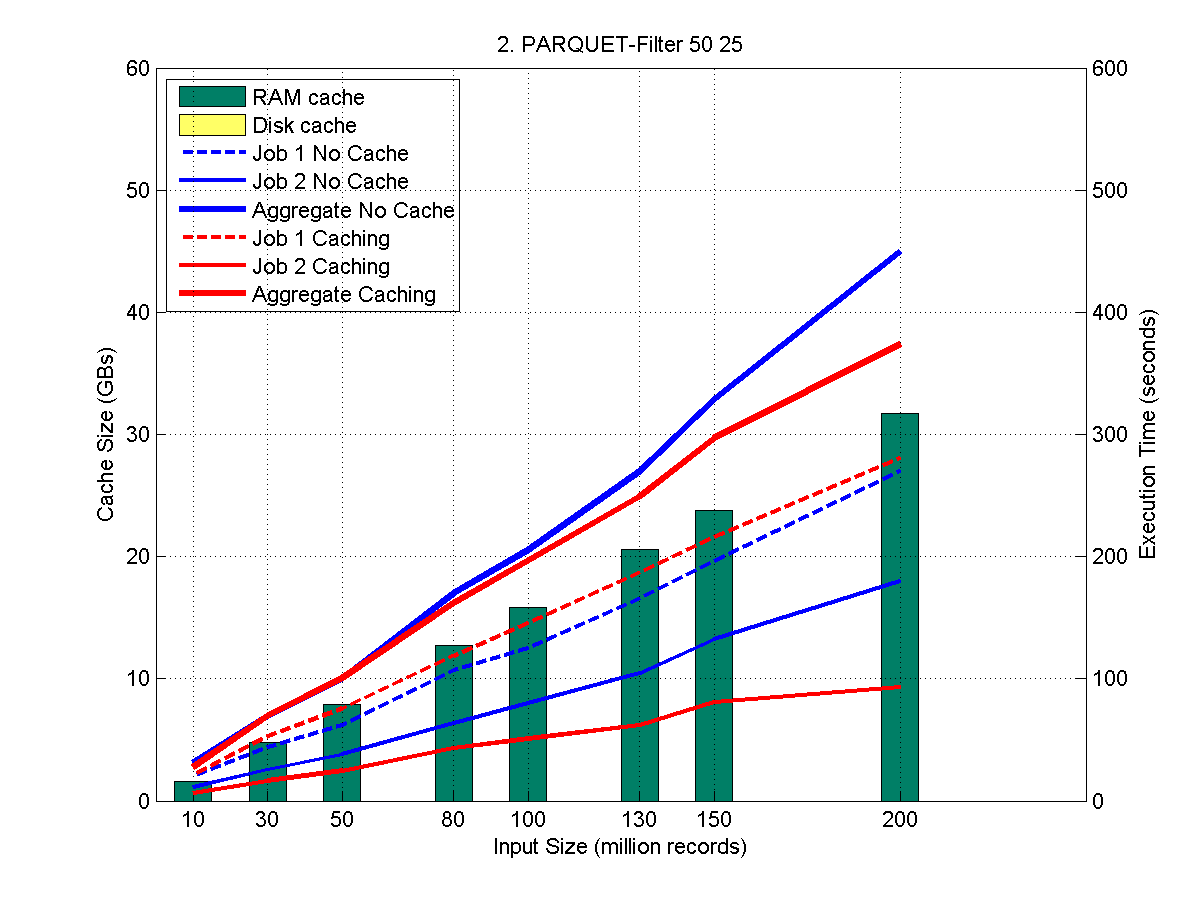
\includegraphics[scale=0.4]{figures/query1_parquet_50}
   \label{fig:query1_parquet_50}}

  	\subfigure[CSV]{
   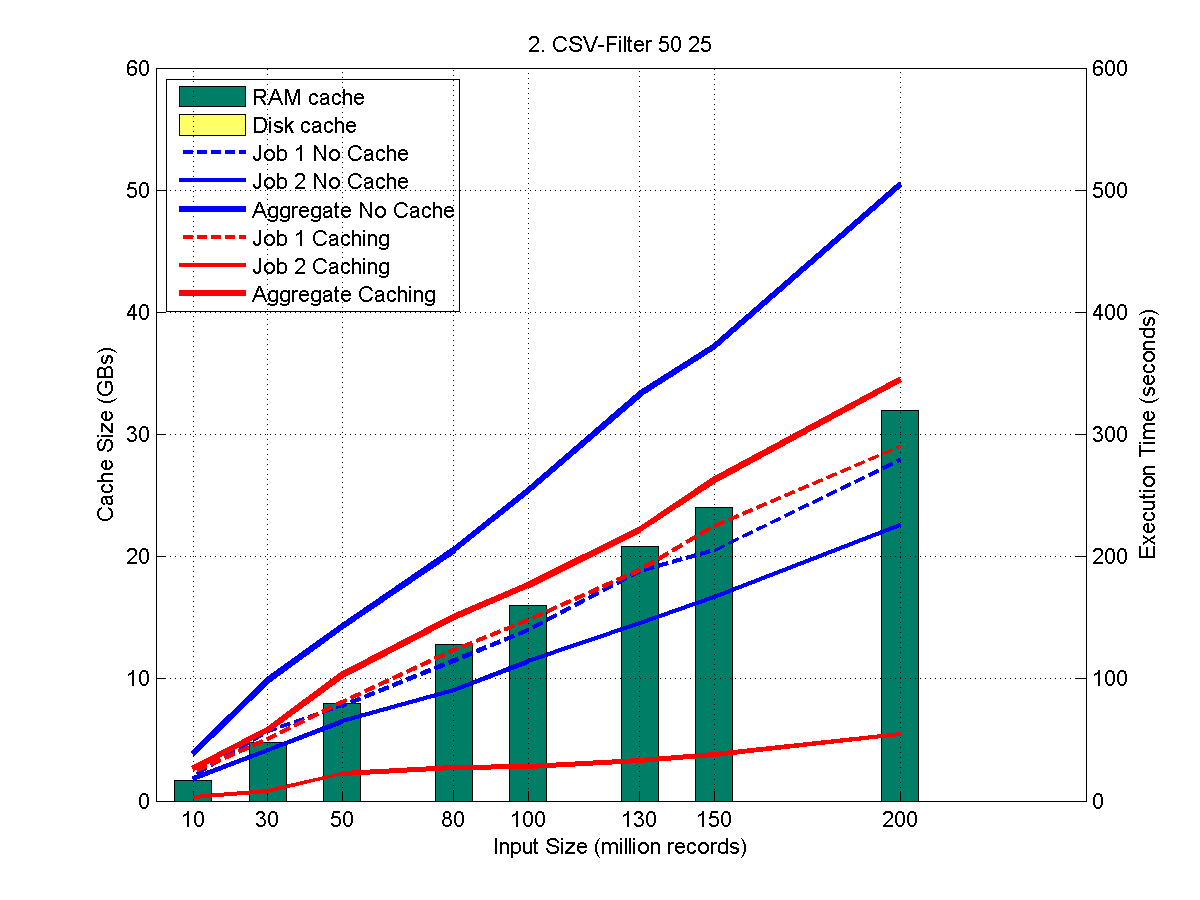
\includegraphics[scale=0.4]{figures/query1_csv_50}
   \label{fig:query1_csv_50}}

   \caption{Filter-based queries, query latencies and memory utilization.}
   \label{fig:query1_50}
\end{figure}

Finally, we consider even less selective predicates, defined as follows: (\texttt{age <= 80} and \texttt{age <= 15}) and (\texttt{age <= 80} and \texttt{age <= 50}). Figures \ref{fig:query1_80_15} and \ref{fig:query1_80_50} show query latencies and memory utilization respectively. For this set of filtering conditions the optimizer caches a lot of data in Job1, of which very little is useful for Job2: as a consequence, the cost of caching might not be balanced by its benefits. This result represents a hint for cost-based optimization: given a set of queries, it is more beneficial to ``pack and cache'' those that have similar cardinalities after applying filtering conditions.

\begin{figure}[htbp]
	\centering

	\subfigure[Parquet]{
   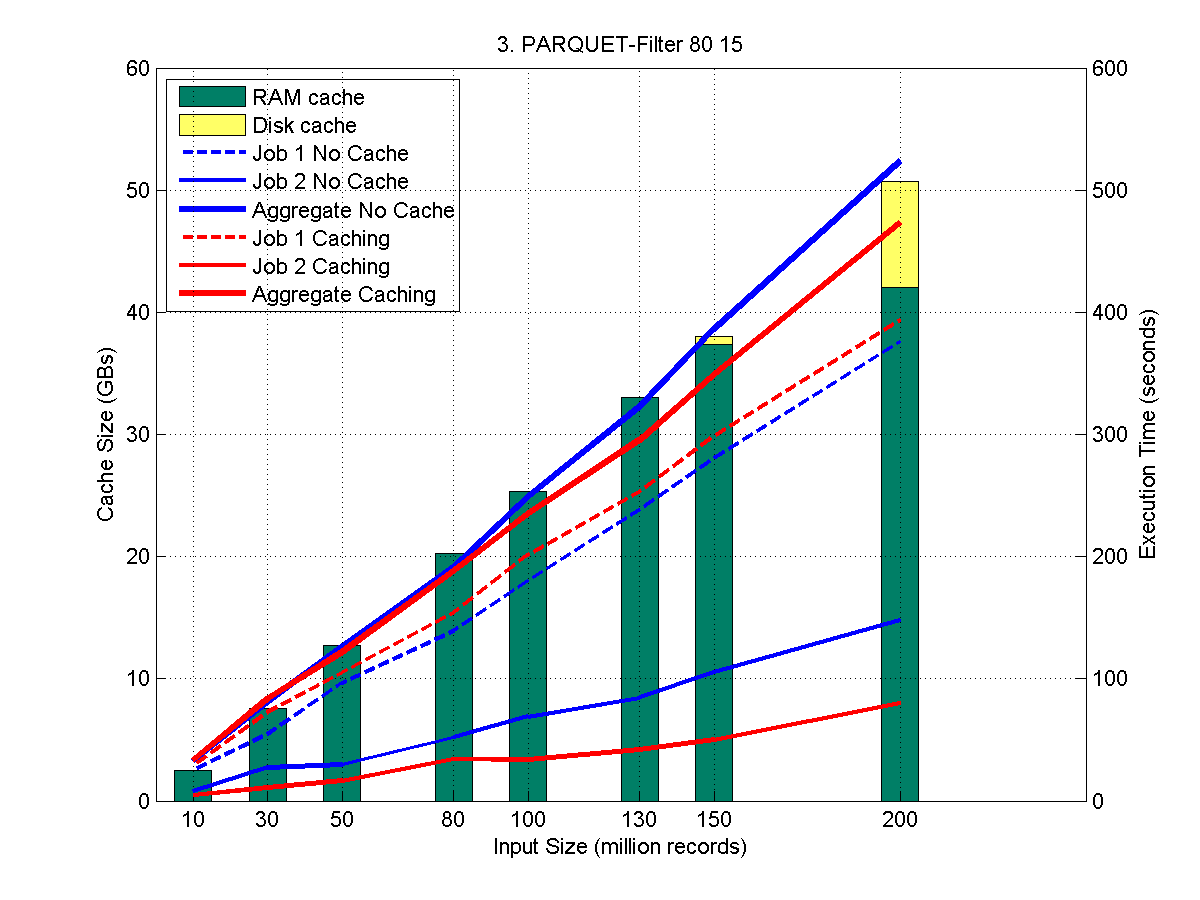
\includegraphics[scale=0.4]{figures/query1_parquet_80_15}
   \label{fig:query1_parquet_80_15}}

  	\subfigure[CSV]{
   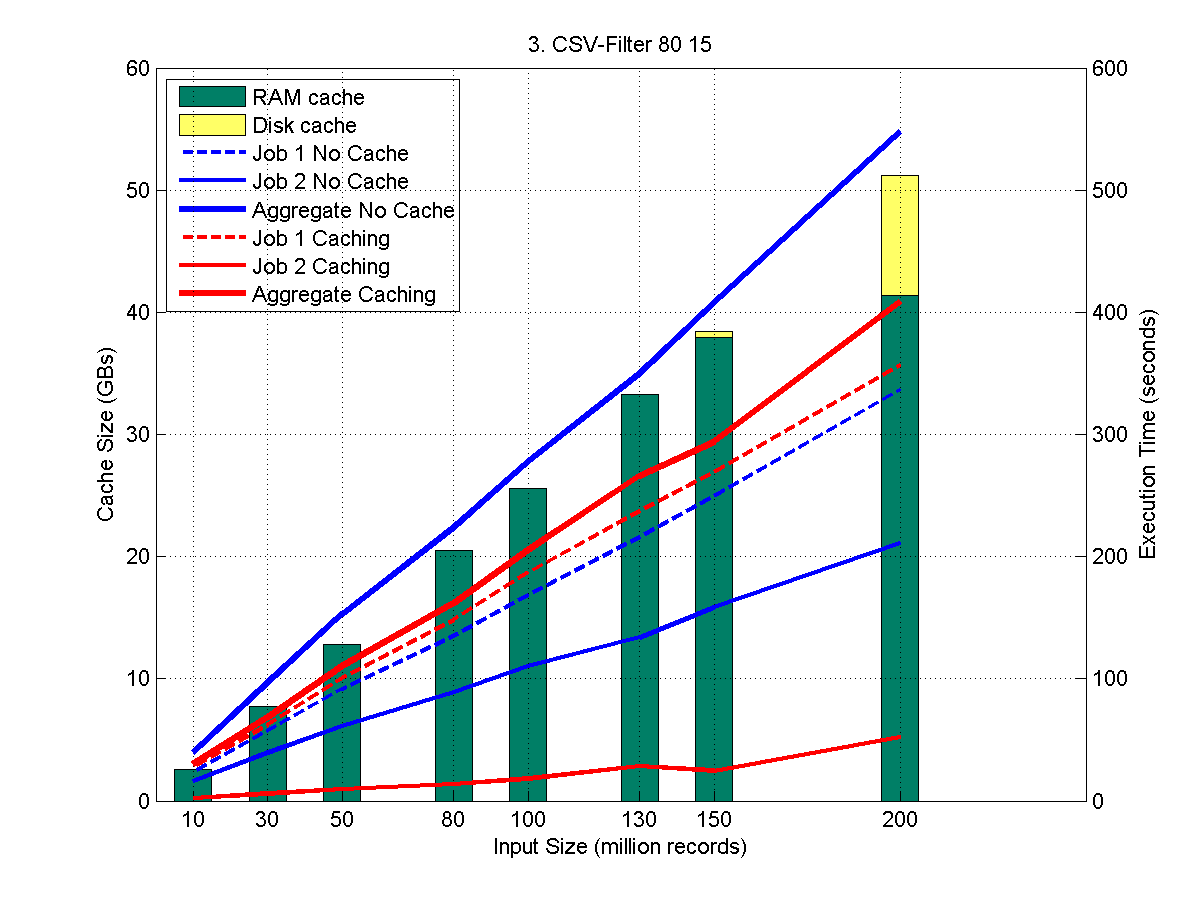
\includegraphics[scale=0.4]{figures/query1_csv_80_15}
   \label{fig:query1_csv_80_15}}

   \caption{Filter-based queries, query latencies and memory utilization.}
   \label{fig:query1_80_15}
\end{figure}

\begin{figure}[htbp]
	\centering

	\subfigure[Parquet]{
   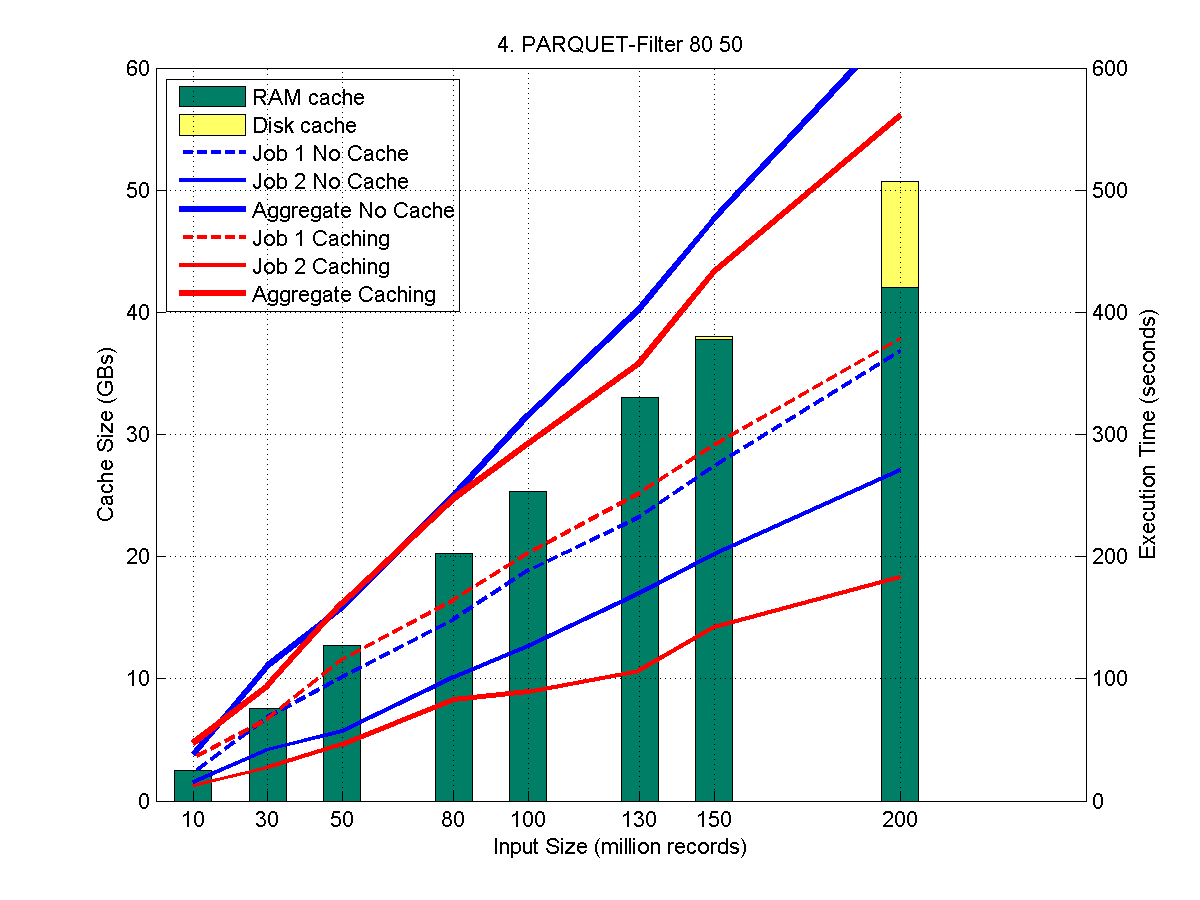
\includegraphics[scale=0.4]{figures/query1_parquet_80_50}
   \label{fig:query1_parquet_80_50}}

  	\subfigure[CSV]{
   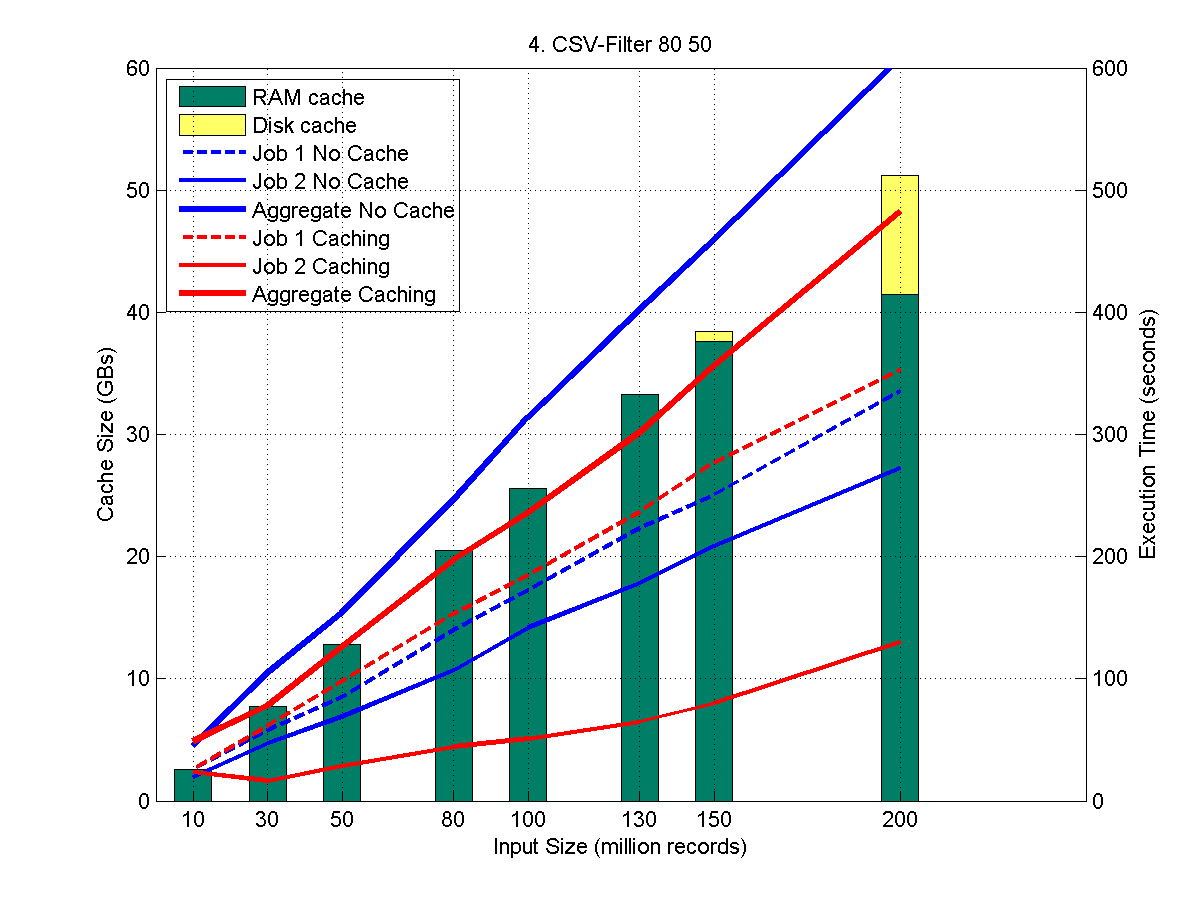
\includegraphics[scale=0.4]{figures/query1_csv_80_50}
   \label{fig:query1_csv_80_50}}

   \caption{Filter-based queries, query latencies and memory utilization.}
   \label{fig:query1_80_50}
\end{figure}


\subsection{Projection-based queries}
Next, we consider simple queries that only perform project operations. Specifically, with reference to the schema of our input data, queries project two attributes: \texttt{desc1:string[100]} and \texttt{desc2:string[200]}.

The original logical plans of the two queries, along with the optimized plan that uses caching are depicted in Figure \ref{fig:query2_plans}.

\begin{figure}[ht]
   \centering
   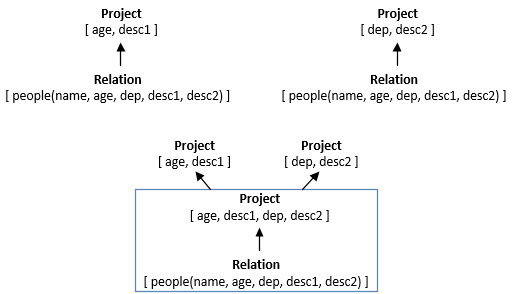
\includegraphics[scale=0.5]{figures/query2_cacheplan}
   \caption{Query and Cache plans for Project-based queries.} 
   \label{fig:query2_plans}
\end{figure}

Next, we present the analysis of the query latencies with and without our optimization, for both Parquet and CSV input data types, in Figures \ref{fig:query2}.

\begin{figure}[ht]
	\centering

	\subfigure[Parquet]{
   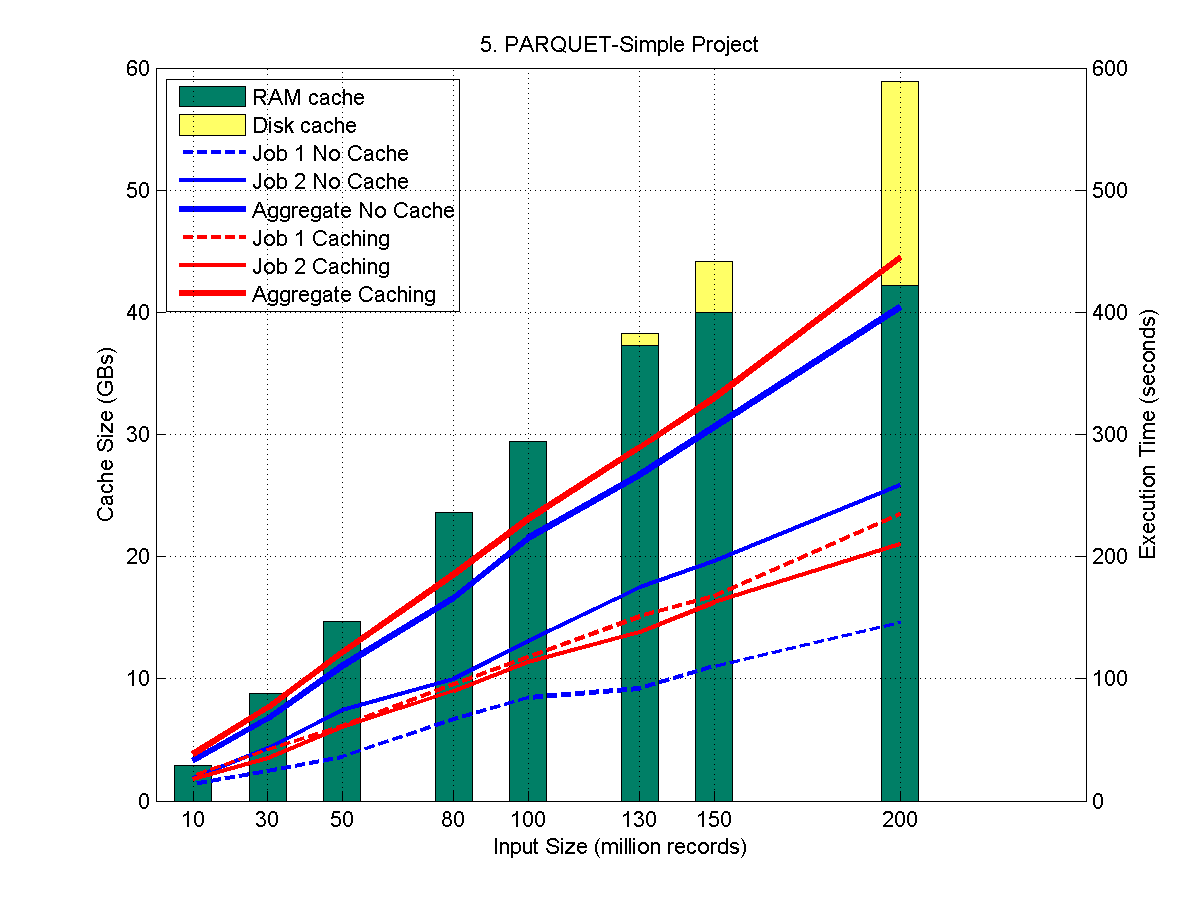
\includegraphics[scale=0.4]{figures/query2_parquet}
   \label{fig:query2_parquet}}

  	\subfigure[CSV]{
   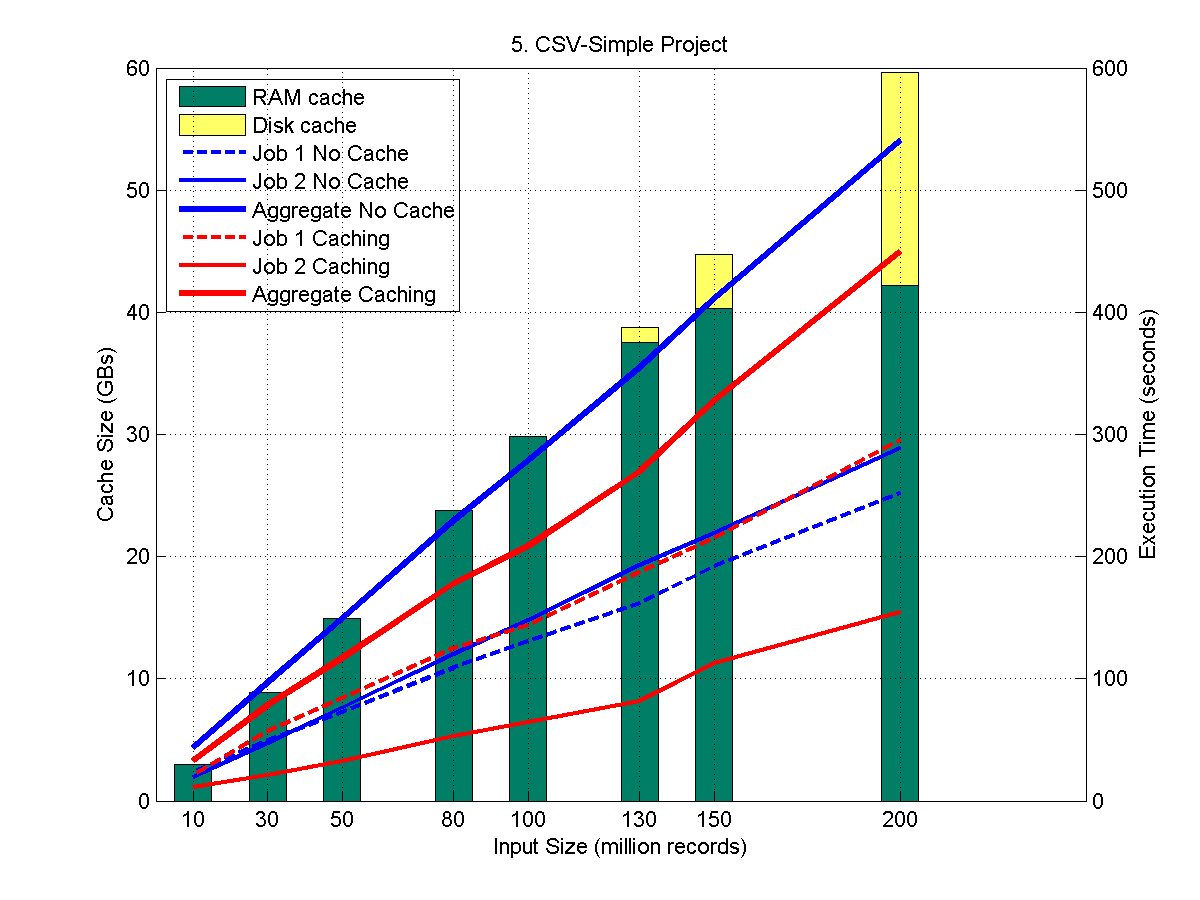
\includegraphics[scale=0.4]{figures/query2_csv}
   \label{fig:query2_csv}}

   \caption{Project-based queries, query latencies and memory utilization.}
   \label{fig:query2}
\end{figure}

Our observations on the results for Project-based queries are as follows. 
When using CSV input data, the benefit of our optimization is clear. Instead, when using the Parquet format, our results indicate little to no benefit in using our optimization. Indeed, Parquet is geared towards columnar data access on disk: as a consequence, the cost associated to cache input data outweighs the benefits of reading two columns from RAM instead of using their disk representations.

\subsection{Projection and Filter based queries}
We now study the impact of our optimization on two queries that mix projection and filters. The logical plans and the optimized plan output by our approach are depicted in Figure \ref{fig:query3_plans}

\begin{figure}[ht]
   \centering
   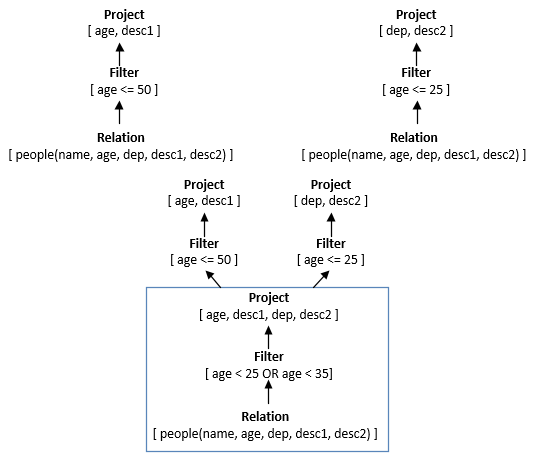
\includegraphics[scale=0.5]{figures/query3_cacheplan}
   \caption{Query and Cache plans for Project and filter based queries.} 
   \label{fig:query3_plans}
\end{figure}

Next, we present the analysis of the query latencies with and without our optimization, for both Parquet and CSV input data types, in Figures \ref{fig:query3}.

\begin{figure}[ht]
	\centering

	\subfigure[Parquet]{
   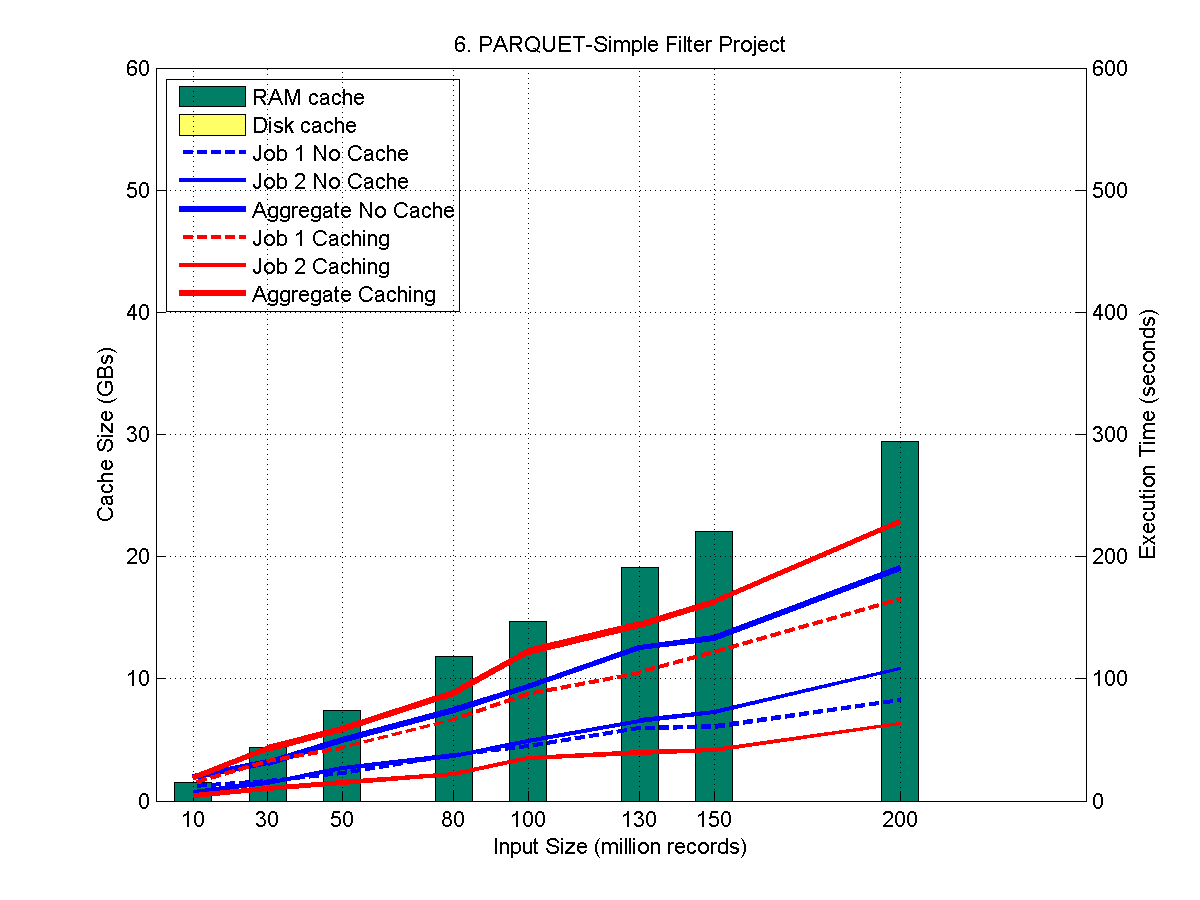
\includegraphics[scale=0.4]{figures/query3_parquet}
   \label{fig:query3_parquet}}

  	\subfigure[CSV]{
   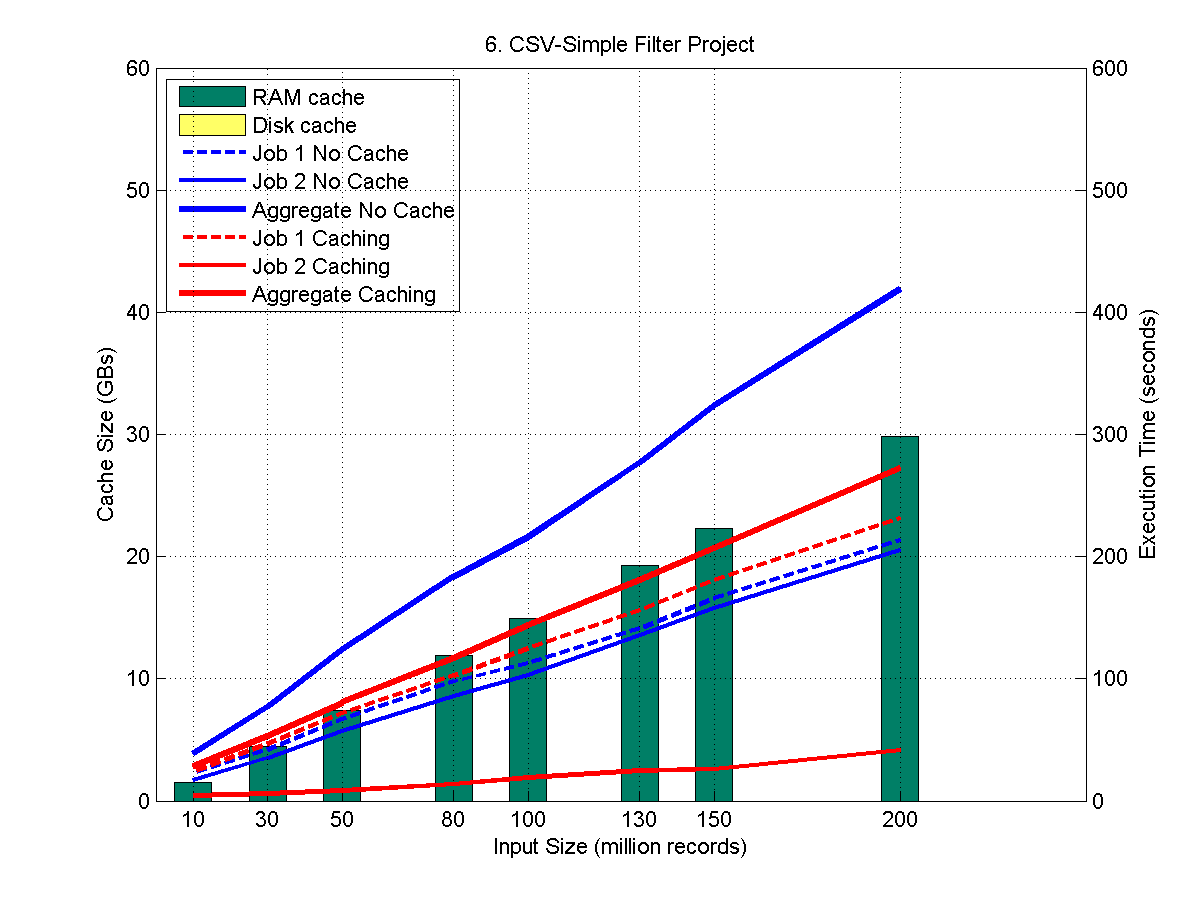
\includegraphics[scale=0.4]{figures/query3_csv}
   \label{fig:query3_csv}}

   \caption{Project-based queries, query latencies and memory utilization.}
   \label{fig:query3}
\end{figure}

Our results indicate that the ``economy'' of our optimization requires a detailed cost-based analysis: in particular, projections on parquet formatted input files do not benefit from caching, and the cost of the cache operation is larger than its benefits.

\subsection{Top-k queries}
We now study consider queries that involve costly processing. In particular, ranking data requires ``shuffling'' data over the network and sorting. The logical plans and the optimized plan output by our approach are depicted in Figure \ref{fig:query4}

\begin{figure}[ht]
   \centering
   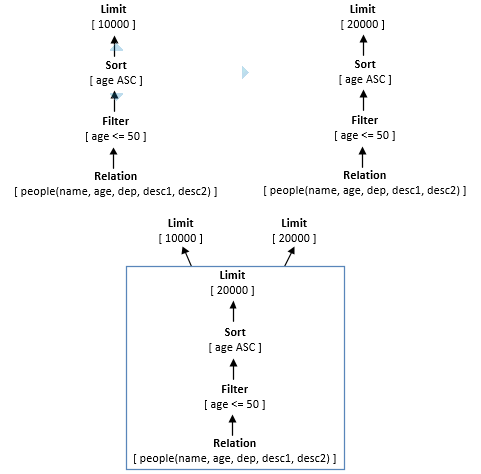
\includegraphics[scale=0.5]{figures/query4_cacheplan}
   \caption{Query and Cache plans for top-k queries.} 
   \label{fig:query4_plans}
\end{figure}

In Figure \ref{fig:query4} we report the query latencies for both Parquet and CSV input data.

\begin{figure}[ht]
	\centering

	\subfigure[Parquet]{
   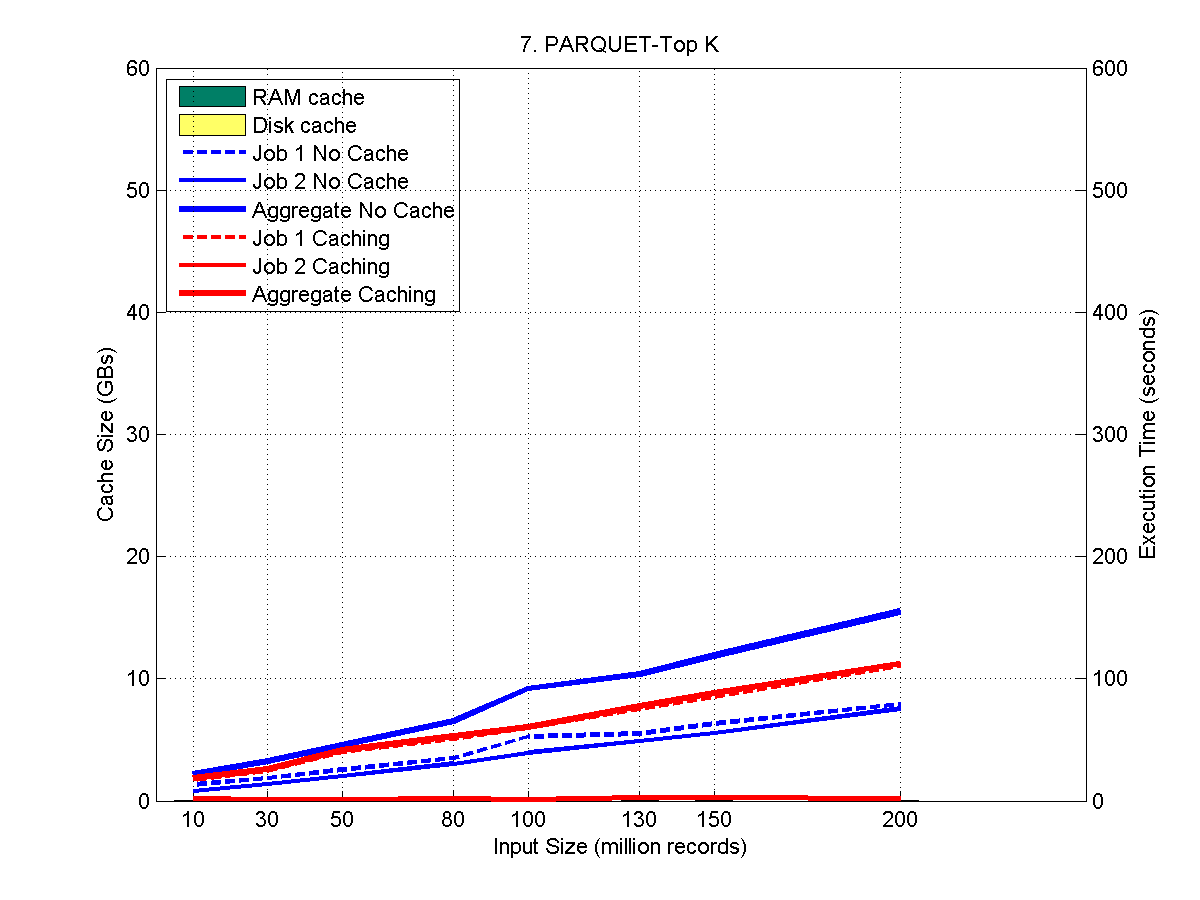
\includegraphics[scale=0.4]{figures/query4_parquet}
   \label{fig:query4_parquet}}

  	\subfigure[CSV]{
   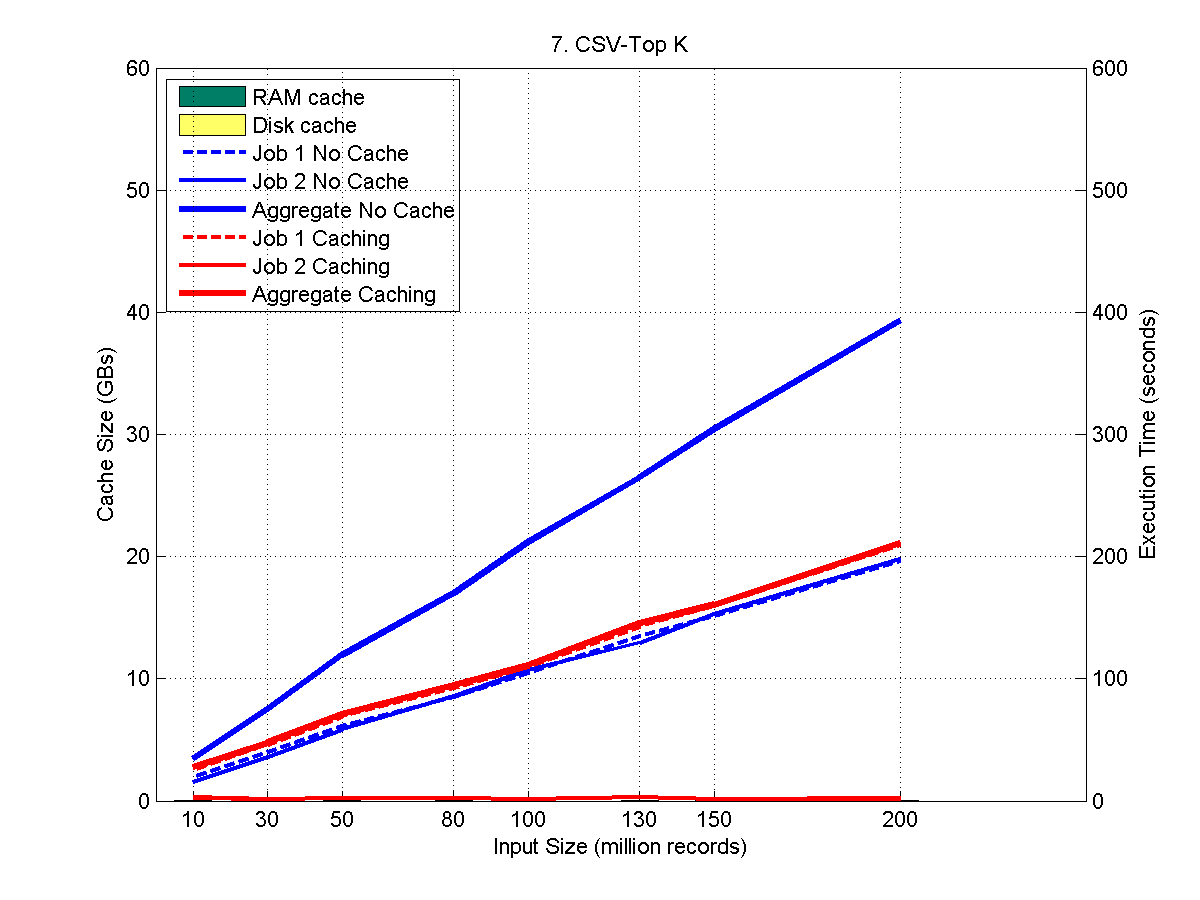
\includegraphics[scale=0.4]{figures/query4_csv}
   \label{fig:query4_csv}}

   \caption{Top-k queries, query latencies and memory utilization.}
   \label{fig:query4}
\end{figure}